\chapter{Grafické uživatelské rozhraní} \label{chap:gui}
    Systém pro simulaci přistávání \acrshort{uav} navržený v~\refskl{chap:system}{kapitole} obsahuje kromě komponent důležitých pro samotnou simulaci také grafické uživatelské rozhraní (\acrshort{gui}), které slouží k~oboustranné komunikaci s~uživatelem před simulací a během ní. Je rozčleněno podle 3 hlavních způsobů užití do 3 obrazovek:
    \begin{enumerate}
        \item Mise (\refskl{sec:mise}{podkapitola}), sloužící k~přípravě misí, správě uložených misí a jejich spouštění.
        \item Živě (\refskl{sec:zive}{podkapitola}), která zobrazuje aktuální data v~průběhu simulace.
        \item Experimenty (\refskl{sec:experimenty}{podkapitola}), jež slouží ke sdružování misí do množin, správě těchto množin a hromadnému spouštění misí z~nich.
    \end{enumerate}
    Mezi obrazovkami se přepíná v~záhlaví nebo pomocí kombinace kláves \Ctrl + \Tab. \acrshort{gui} je implementováno v~programovacím jazyce Python pomocí bindingů frameworku Qt do Pythonu zvaného PyQt \cite{pyqt}.
    \section{Obrazovka Mise} \label{sec:mise}
    \begin{figure}
        \centering
        \begin{tikzpicture}[execute at end picture={
    % \draw (current bounding box.south west)
    %     grid [step=0.5cm] (current bounding box.north east);
}]
    \node[inner sep=0pt, above right] (screen) at (0,0) {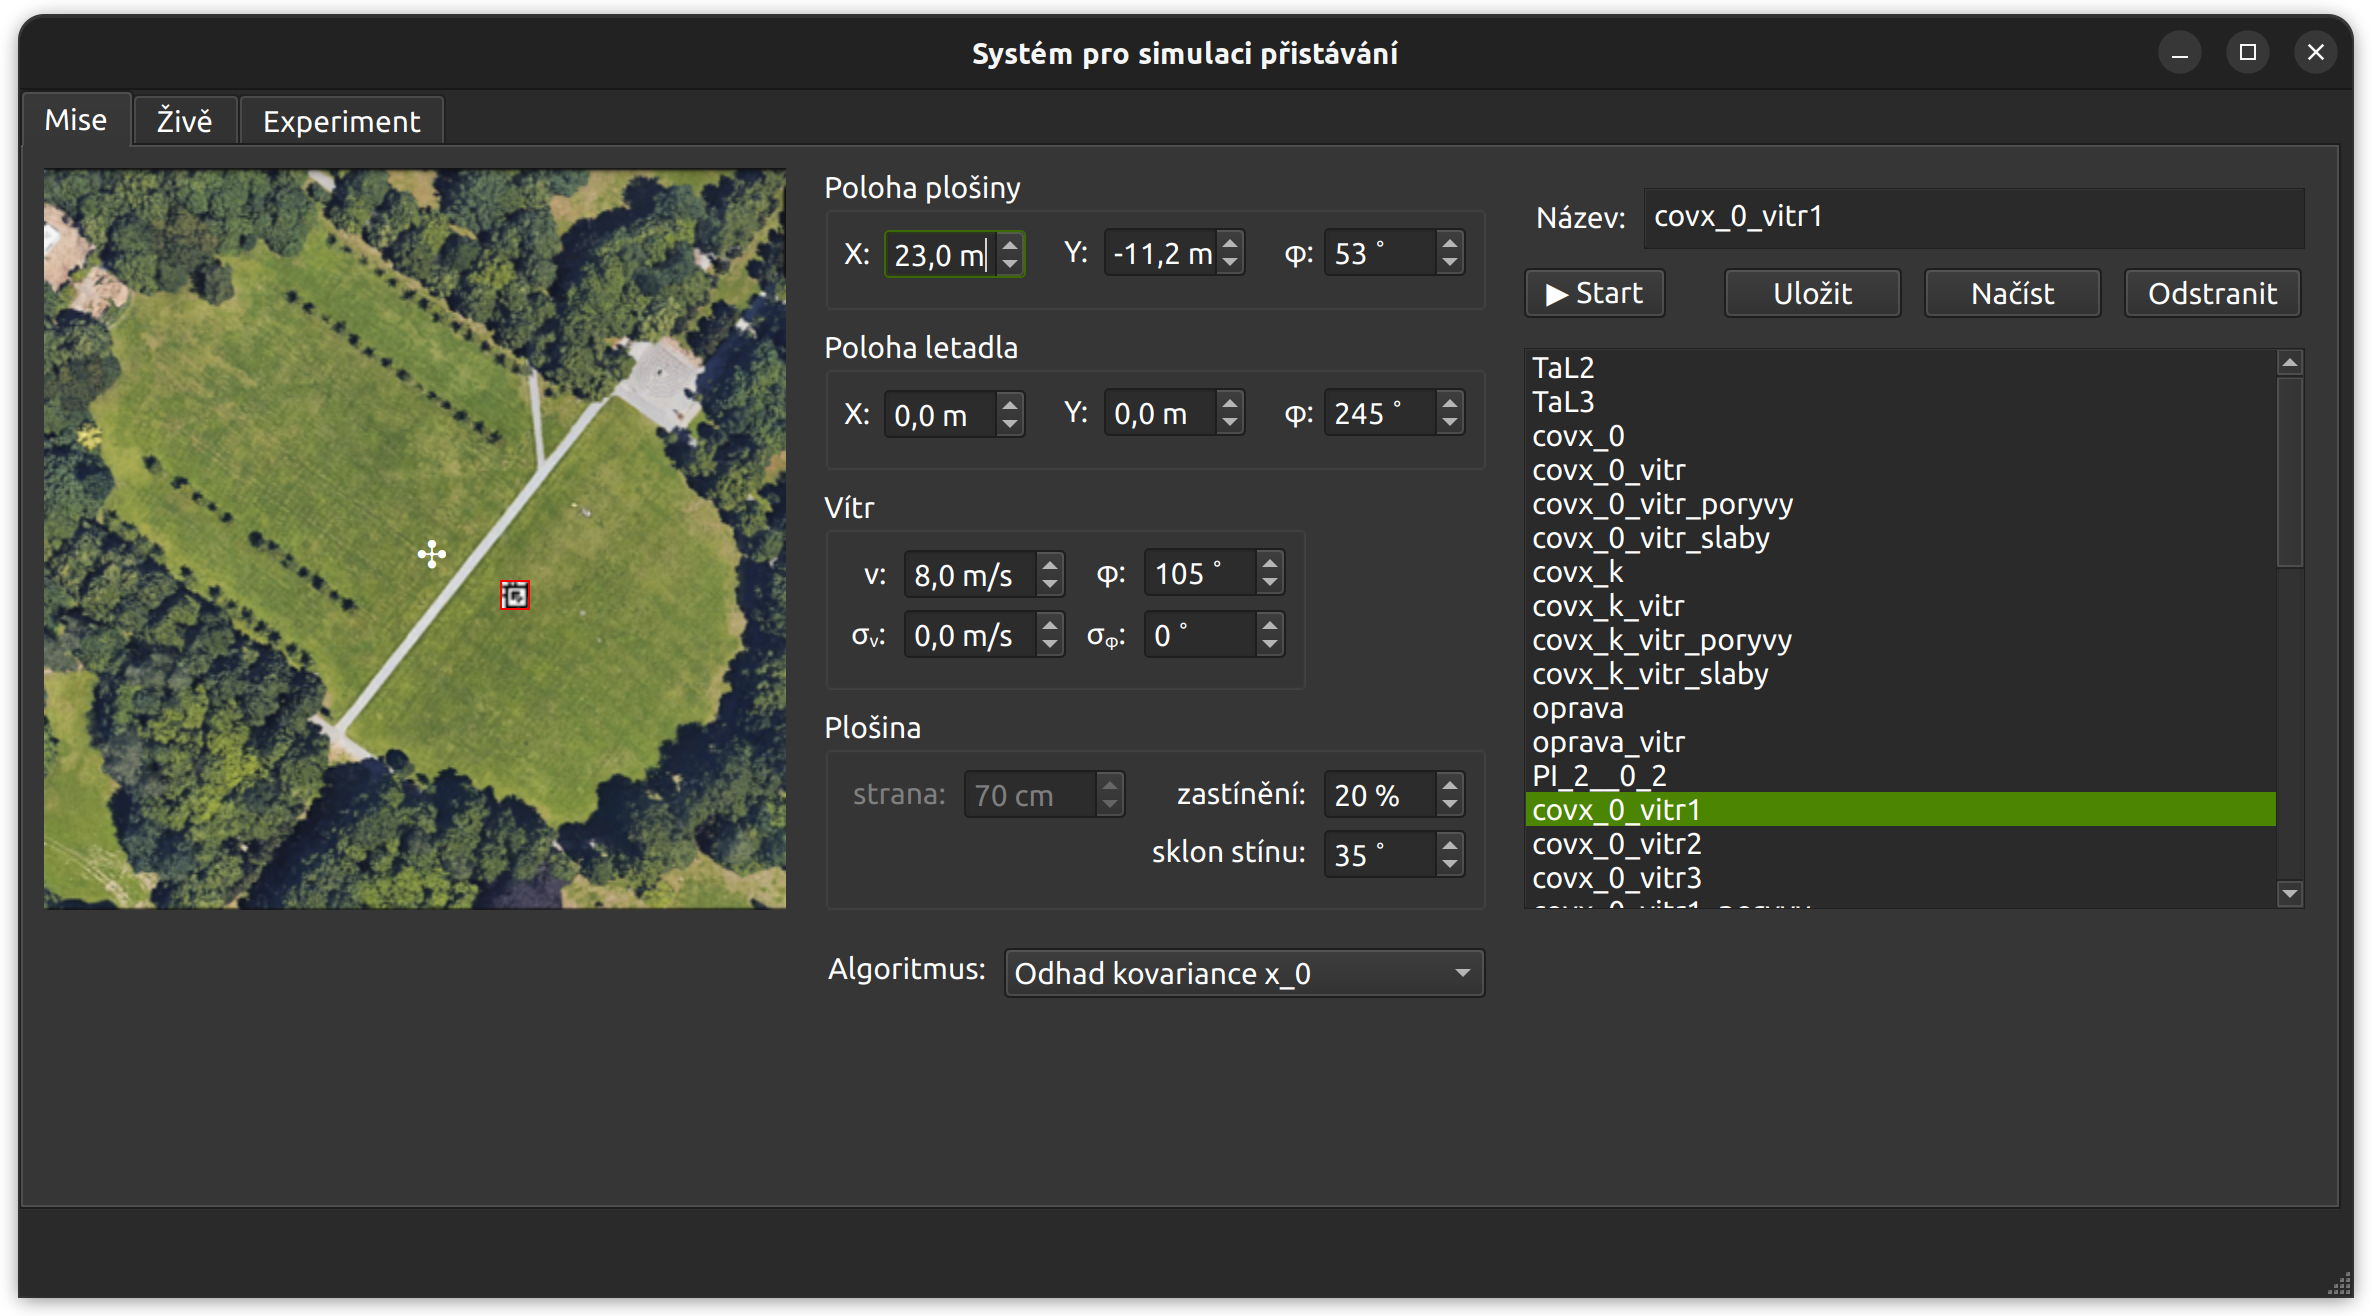
\includegraphics[width=\textwidth]{gui/mise.png}};

    \node[draw, above right, minimum height=4.68cm, minimum width=4.68cm, color=red, line width=1pt, pin={[pin={[pin distance=0cm,draw,circle,node font=\tiny,pin edge={red}]right:2},pin distance=1.55cm, pin edge={red}]83:Mapa}] (mapa) at (0.25,2.5) {};

    \node[draw, below right, minimum height=0.43cm, minimum width=4.32cm, color=purple, line width=1pt, pin={[pin={[pin distance=0cm,draw,circle,node font=\tiny,pin edge={red}]left:7},pin distance=3cm, pin edge={red}]below:Výběr metody přistávání}] (alg) at (5.05,2.4) {};
    \node[draw, above right, minimum height=1.35cm, minimum width=4.32cm, color=magenta, line width=1pt, pin={[pin={[pin distance=0cm,draw,circle,node font=\tiny,pin edge={magenta}]left:6},pin distance=3cm, pin edge={magenta}]260:Vlastnosti plošiny}] (plosina) at (5.05,2.45) {};
    \node[draw, above right, minimum height=1.33cm, minimum width=4.32cm, color=cyan, line width=1pt, pin={[pin={[pin distance=0cm,draw,circle,node font=\tiny,pin edge={cyan}]left:5},pin distance=4cm, pin edge={cyan}]280:Nastavení větru}] (vitr) at (5.05,3.87) {};
    \node[draw, above right, minimum height=0.95cm, minimum width=4.32cm, color=blue, line width=1pt, pin={[pin={[pin distance=0cm,draw,circle,node font=\tiny,pin edge={blue}]left:3},pin distance=2.3cm, pin edge={blue}]105:Umístění plošiny}] (plosinaPoloha) at (5.05,6.25) {};
    \node[draw, above right, minimum height=0.95cm, minimum width=4.32cm, color=orange, line width=1pt, pin={[pin={[pin distance=0cm,draw,circle,node font=\tiny,pin edge={orange}]above:4},pin distance=2.57cm, pin edge={orange}]88:Umístění letounu}] (uav) at (5.05,5.25) {};

    \node[draw, above right, minimum height=3.65cm, minimum width=5.15cm, color=red, line width=1pt, pin={[pin={[pin distance=0cm,draw,circle,node font=\tiny,pin edge={red}]left:9},pin distance=3.5cm, pin edge={red}]below:Uložené mise}] (mise) at (9.47,2.45) {};
    \node[draw, above right, minimum height=1cm, minimum width=5.15cm, color=green, line width=1pt, pin={[pin={[pin distance=0cm,draw,circle,node font=\tiny,pin edge={green}]left:8},pin distance=1.58cm, pin edge={green}]above:Práce s misí}] (tlacitka) at (9.47,6.2) {};

    \node[draw, above right, minimum height=0.47cm, minimum width=2.77cm, color=green, line width=1pt, pin={[pin={[pin distance=0cm,draw,circle,node font=\tiny,pin edge={green}]above:1},pin distance=1cm, pin edge={green}]above:Výběr obrazovky}] (zalozky) at (0.06,7.25) {};
\end{tikzpicture}
        \caption[GUI: Obrazovka \uv{Mise}]{Obrazovka \uv{Mise} grafického uživatelského rozhraní navrhovaného systému pro simulaci přistávání bezpilotního letadla. Slouží k~definici vlastností simulace, ukládání definic a spouštění simulace s~danými podmínkami.}
        \label{fig:tabMise}
    \end{figure}
    Mise je první ze 3 obrazovek \acrshort{gui} navrhovaného systému (\cref{chap:system}), pomocí níž je možné definovat mise pro simulaci, zobrazovat je na mapě, ukládat a spouštět. K~jednotlivým úkonům slouží různé její části (v~\refskl{fig:tabMise}{obrázku} označené \kolecko{1} - \kolecko{9}), které budou dále popsány. Mezi ovládacími prvky se lze pohybovat pomocí klávesy tabulátoru.
    \paragraph{\kolecko{1} Výběr obrazovky.}Jak již bylo zmíněno, celé \acrshort{gui} je členěno do 3 obrazovek. V~levém horním rohu každé z~nich jsou po celou dobu běhu programu umístěny 3 záložky, které reprezentují jednotlivé obrazovky (Mise, Živě, Experimenty). Záložka právě nahlížené obrazovky je zvýrazněna světlejším provedením a je graficky spojena se spodní částí rozhraní. V~podkapitolách o~dalších obrazovkách (\cref*{sec:zive,sec:experimenty}) již tento výběr není zmiňován, protože je společný.

    \paragraph{\kolecko{2} Mapa}vizualizuje polohu plošiny nastavenou ve střední části obrazovky (\kolecko{3}) pomocí jejího obrázku s~červenou hranou a polohu letounu (zadanou v~části \kolecko{4}) pomocí bílého kříže s~kruhy na všech ramenou, který tak připomíná kvadrokoptéru, na leteckém snímku použitém v~simulátoru jako podklad.

    \paragraph{\kolecko{3} Umístění plošiny} umožňuje nastavit souřadnice $X$ a $Y$ středu plošiny vzhledem k~počátku simulovaného světa, který se nachází uprostřed mapy, a úhel natočení $\phi$ vůči ose $x$. Změna polohy aktualizuje vizualizaci v~mapě (\kolecko{2}).

    \paragraph{\kolecko{4} Umístění letounu} poskytuje stejná nastavení ($X, Y, \phi$) pro letoun jako část \kolecko{3} pro plošinu. Nastavené hodnoty reflektuje ikona dronu v~mapě (\kolecko{2}).

    \paragraph{\kolecko{5} Nastavení větru} zahrnuje 4 proměnné, které ovlivňují působení větru na model v~simulaci. Jedná se o~vodorovnou rychlost a její směrodatnou odchylku ($v$ a $\sigma_v$) a vodorovný úhel vzhledem k~ose $x$ a jeho směrodatnou odchylku ($\phi$ a $\sigma_\phi$). Tyto hodnoty se pak využívají při generování definičního souboru světa pro nastavení vlastností pluginu, který generuje okamžité vlastnosti větru v~každém kroku simulace.

    \paragraph{\kolecko{6} Vlastnosti plošiny} dává možnosti nastavení dalších aspektů simulované plošiny, tedy její velikosti (možnost strana), podílu zastíněné části úsečky vedené středem plošiny ve směru osy $y$ a sklonu stínu. \Cref{fig:stin} ukazuje příklad simulace přistávání letounu na částečně zastíněnou plošinu.
    \begin{figure}
        \centering
        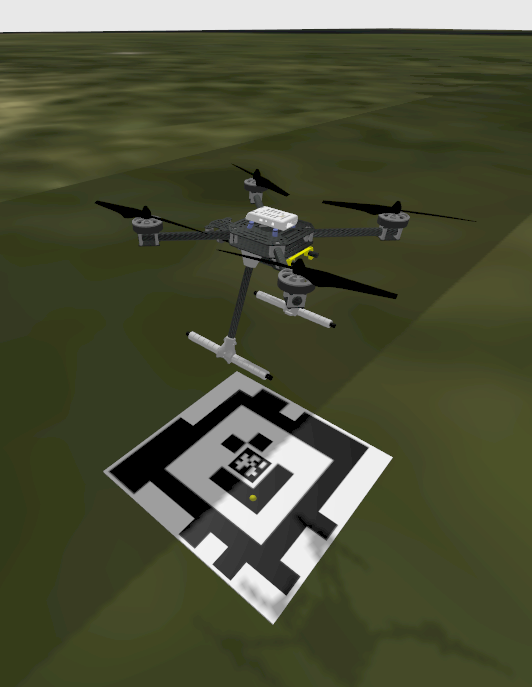
\includegraphics[width=0.3\textwidth]{img/gui/stin.png}
        \caption[Přistávání na zastíněnou plošinu]{Příklad simulace přistávání bezpilotního letounu na plošinu s~fiduciárním markerem, která je částečně zastíněná.}
        \label{fig:stin}
    \end{figure}

    \paragraph{\kolecko{7} Výběr metody přistávání}umožňuje uživateli z~nabídky vybrat algoritmus, který se použije k~řízení \acrshort{uav} během simulace. Metody v~nabídce jsou předdefinované a uživatelsky je nelze měnit. Vlastnosti některých metod je možné upravit změnou konfiguračního souboru.

    \paragraph{\kolecko{8} Práce s~misí} je část obrazovky, pomocí níž se nastavuje název mise, definice jím identifikovaná se dá uložit do seznamu, načíst z~něj (což přepíše aktuální hodnoty v~částech \kolecko{2} - \kolecko{7}) nebo odstranit. Aktuálně nastavené hodnoty v~předchozích částech pak mohou být využity pro spuštění simulace, kdy se název mise zároveň použije jako název světa a nedodá-li ho uživatel, je použita výchozí hodnota \uv{BezNazvu}.

    \paragraph{\kolecko{9} Uložené mise} zobrazuje seznam názvů dříve uložených definic misí. Ty se uchovávají v~souboru načítaném při spuštění programu. Spravovat je lze pomocí ovládacích prvků v~části \kolecko{8}.
    
    \section{Obrazovka Živě} \label{sec:zive}
        \begin{figure}
            \centering
            \begin{tikzpicture}[execute at end picture={
    % \draw (current bounding box.south west)
    %     grid [step=0.5cm] (current bounding box.north east);
}]
    \node[inner sep=0pt, above right] (screen) at (0,0) {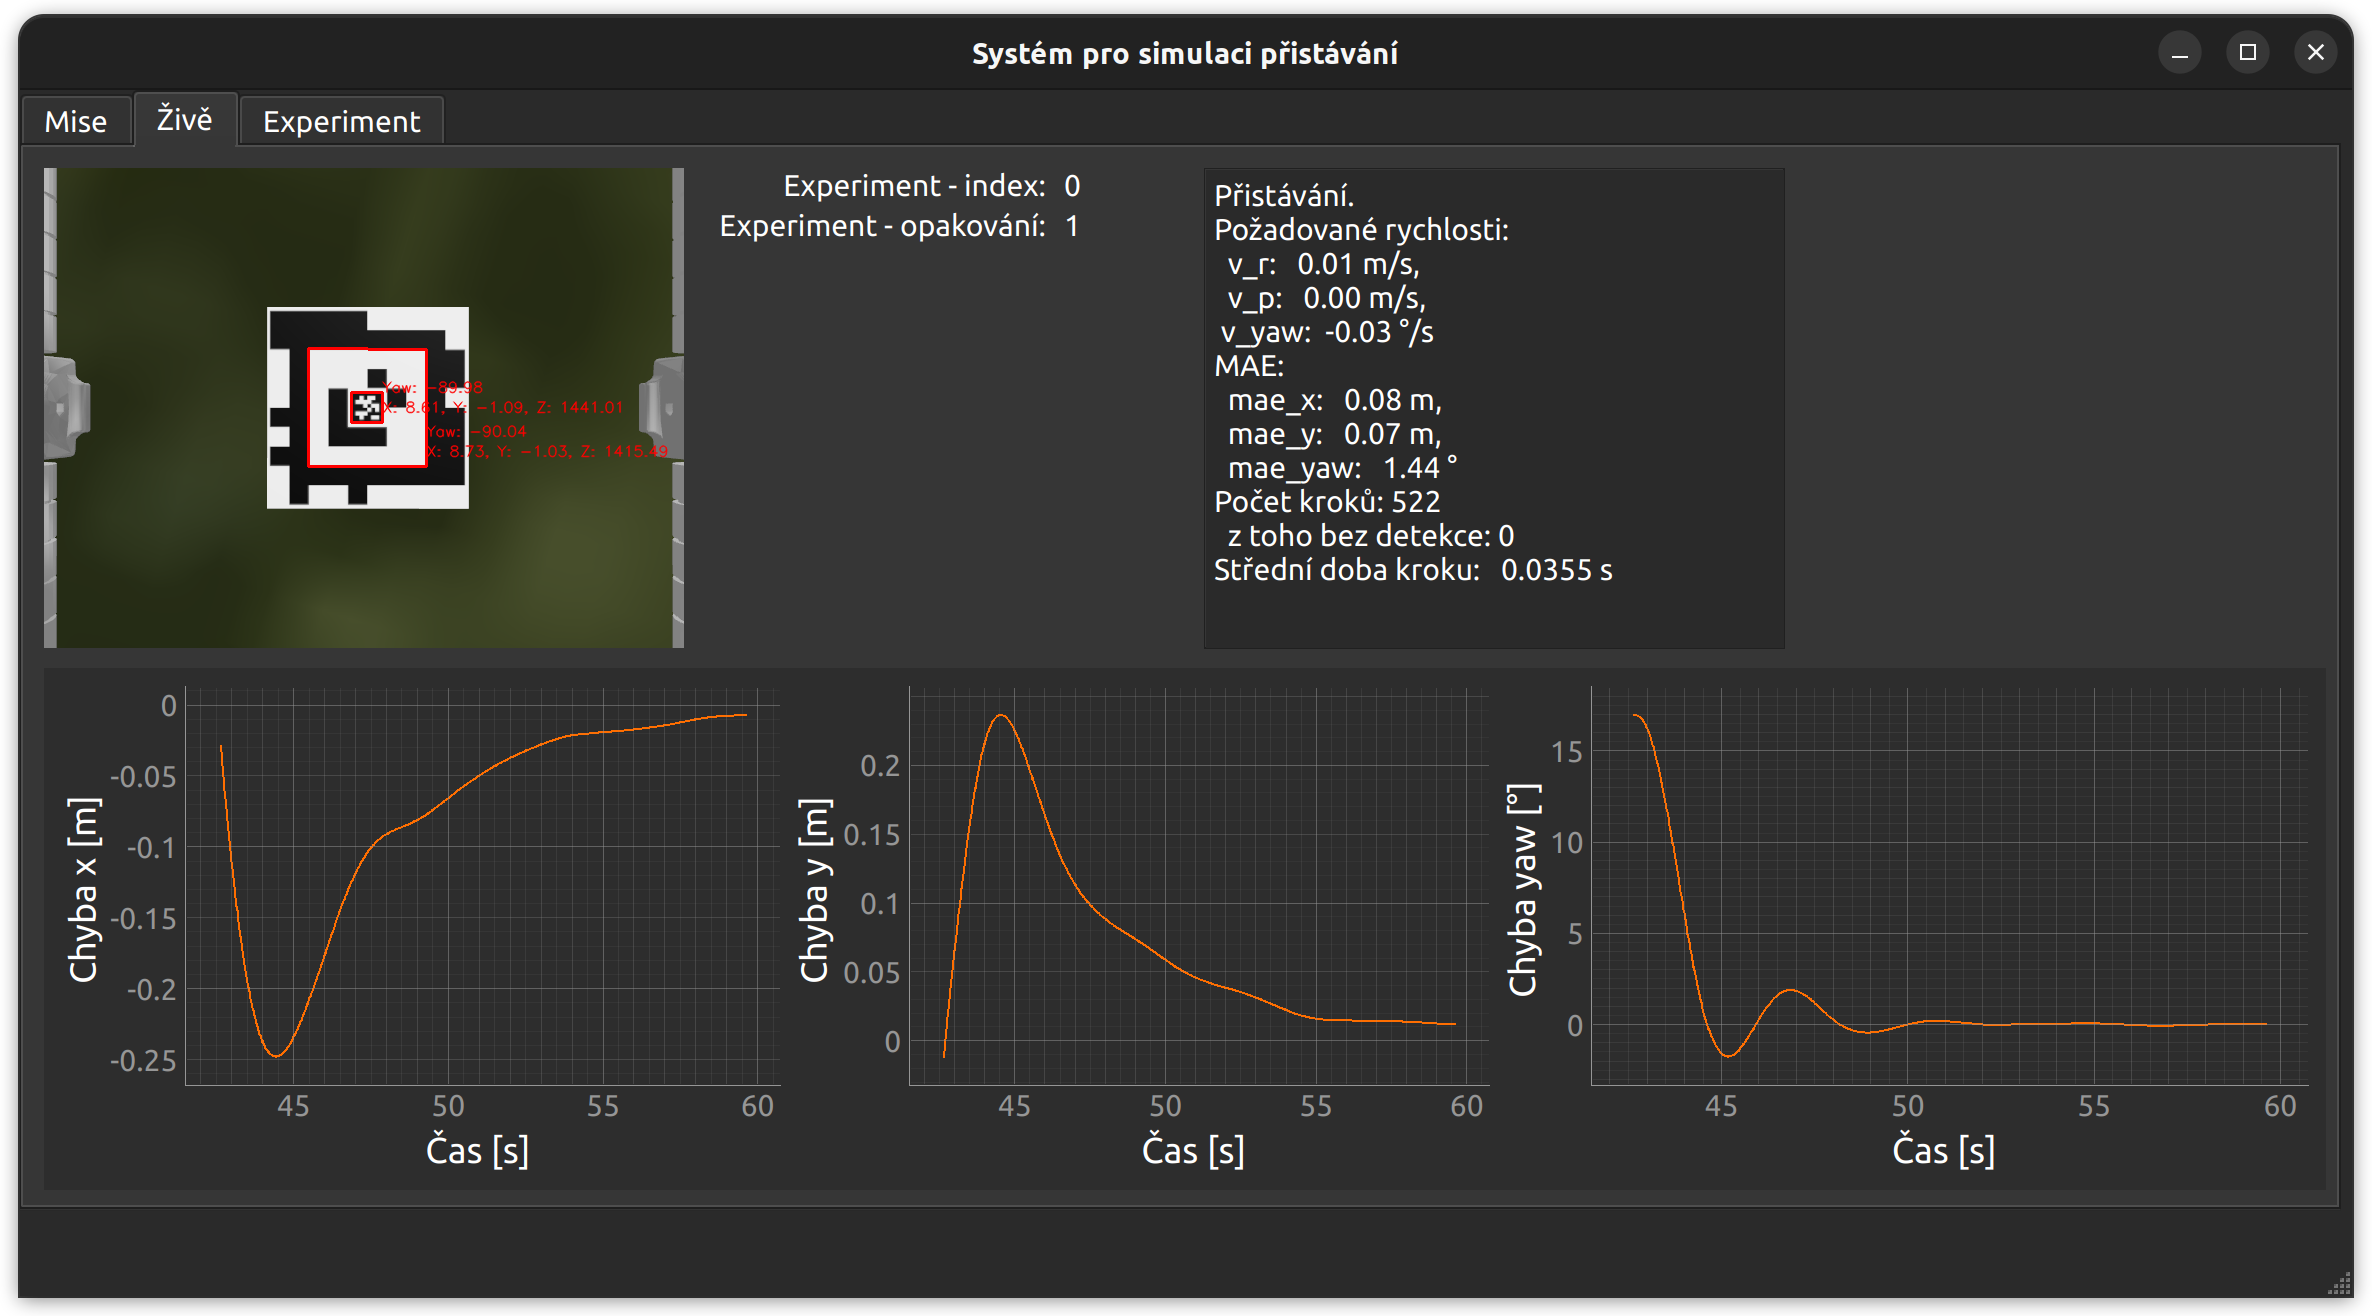
\includegraphics[width=\textwidth]{gui/live (2).png}};

    \node[draw, above right, minimum height=3cm, minimum width=4.05cm, color=red, line width=1pt, pin={[pin={[pin distance=0cm,draw,circle,node font=\tiny,pin edge={red}]left:2},pin distance=2.1cm, pin edge={red}]75:Pohled kamery}] (kamera) at (0.25,4.2) {};

    \node[draw, above right, minimum height=3.2cm, minimum width=14.5cm, color=cyan, line width=1pt, pin={[pin={[pin distance=0cm,draw,circle,node font=\tiny,pin edge={cyan}]left:5},pin distance=1.2cm, pin edge={cyan}]below:Grafy chyb}] (grafy) at (0.25,0.75) {};
    \node[draw, above right, minimum height=0.5cm, minimum width=2.4cm, color=blue, line width=1pt, pin={[pin={[pin distance=0cm,draw,circle,node font=\tiny,pin edge={blue}]left:3},pin distance=1.6cm, pin edge={blue}]80:Informace o experimentu}] (expInfo) at (4.45,6.7) {};
    \node[draw, above right, minimum height=3cm, minimum width=3.75cm, color=orange, line width=1pt, pin={[pin={[pin distance=0cm,draw,circle,node font=\tiny,pin edge={orange}]left:4},pin distance=2cm, pin edge={orange}]55:Stav algoritmu}] (alg) at (7.55,4.15) {};

    \node[draw, above right, minimum height=0.47cm, minimum width=2.77cm, color=green, line width=1pt, pin={[pin={[pin distance=0cm,draw,circle,node font=\tiny,pin edge={green}]above:1},pin distance=1cm, pin edge={green}]above:Výběr obrazovky}] (zalozky) at (0.06,7.25) {};
\end{tikzpicture}
            \caption[GUI: Obrazovka \uv{Živě}]{Obrazovka \uv{Živě} grafického uživatelského rozhraní navrhovaného systému pro simulaci přistávání bezpilotního letadla. Slouží k~dohledu uživatele na simulaci.}
            \label{fig:tabZive}
        \end{figure}
        Druhou ze 3 obrazovek \acrshort{gui} navrhovaného systému (\cref{chap:system}) je obrazovka Živě, která uživateli zprostředkovává informace o~právě probíhající simulaci. Jedná se o~pohled z~kamery, informace o~experimentu (je-li nějaký spuštěn), výpis stavu poskytovaný algoritmem a grafy chyb v~poloze a natočení vůči plošině. Snímek této obrazovky je na \refskl{fig:tabZive}{obrázku}.

        \paragraph{\kolecko{2} Pohled kamery} se nachází v~levém horním rohu obrazovky a jedná se o~obraz získávaný z~kamery, která je svázaná se simulovaným modelem. Pokud je v~jejím zorném poli detekován marker, je označen červeným rámem a jsou k~němu připojeny informace o~jeho poloze vůči dronu.

        \paragraph{\kolecko{3} Informace o~experimentu} zahrnují index probíhající mise a počet již proběhlých opakování této mise. Index odpovídá pořadí v~tabulce na obrazovce Experimenty. Pokud žádný experiment neprobíhá, zobrazují se místo těchto informací pomlčky v~příslušných polích.

        \paragraph{\kolecko{4} Stav algoritmu} je text v~přirozeném jazyce, který poskytuje algoritmus jako shrnutí svého stavu v~daném okamžiku. Pro implementované metody se během přistávání jedná o~požadované rychlosti vodorovně vpravo, vpřed a kolem svislé osy dronu, \acrshort{mae} v~souřadnicích $x$, $y$ a rotaci kolem svislé osy, počtu již proběhlých kroků algoritmu a střední doby kroku.

        \paragraph{\kolecko{5} Grafy chyb.} Spodní polovinu obrazovky zaujímají 3 grafy, ve kterých je vykreslen průběh chyby v~souřadnicích $x$ a $y$ a rotaci kolem svislé osy v~závislosti na čase. Chybou se rozumí rozdíl skutečnou a požadovanou trajektorií. Grafy jsou interaktivní, je možné přiblížení a oddálení pomocí kolečka myši a pohyb tahem kurzoru, kdy osa $x$ všech grafů je svázána. Vrátit se do půbodního zobrazení je možné pomocí tlačítka, které se zobrazí v~levém dolním rohu grafu při změně.
    \section{Obrazovka Experimenty} \label{sec:experimenty}
        \begin{figure}
            \centering
            \begin{tikzpicture}[execute at end picture={
    % \draw (current bounding box.south west)
    %     grid [step=0.5cm] (current bounding box.north east);
}]
    \node[inner sep=0pt, above right] (screen) at (0,0) {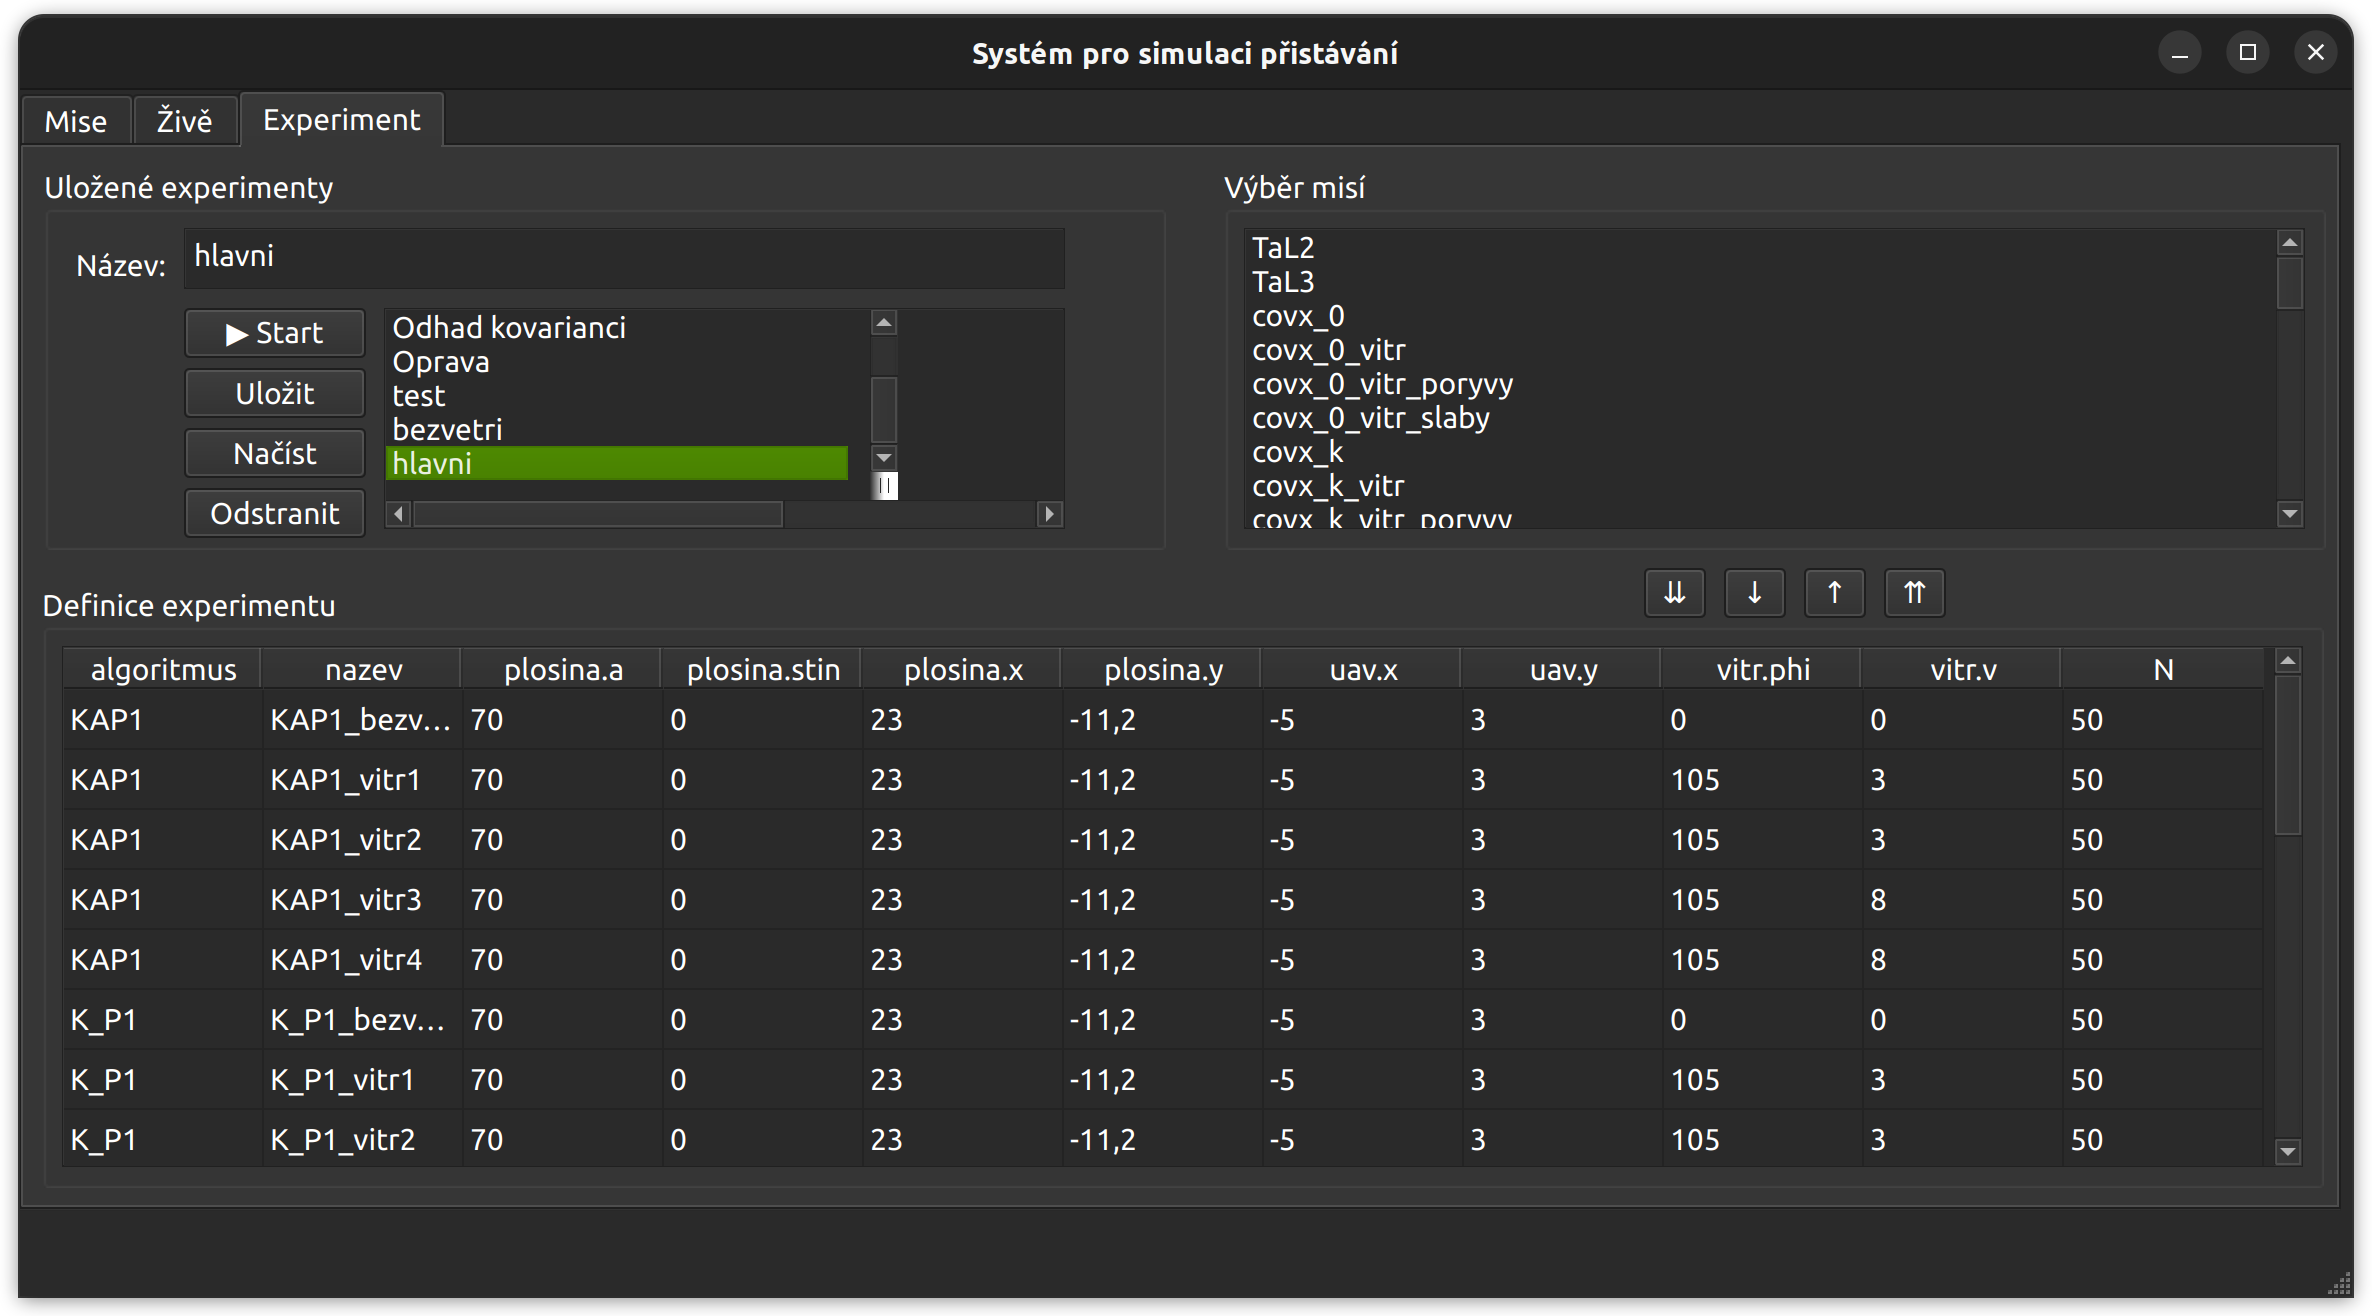
\includegraphics[width=\textwidth]{gui/experimenty.png}};

    \node[draw, above right, minimum height=2.5cm, minimum width=7.2cm, color=red, line width=1pt, pin={[pin={[pin distance=0cm,draw,circle,node font=\tiny,pin edge={red}]left:2},pin distance=1.57cm, pin edge={red}]75:Správa experimentů}] (exp) at (0.20,4.7) {};

    \node[draw, above right, minimum height=3.6cm, minimum width=14.5cm, color=cyan, line width=1pt, pin={[pin={[pin distance=0cm,draw,circle,node font=\tiny,pin edge={cyan}]left:4},pin distance=1.2cm, pin edge={cyan}]below:Definice experimentu}] (grafy) at (0.2,0.6) {};
    \node[draw, above right, minimum height=3cm, minimum width=7.15cm, color=orange, line width=1pt, pin={[pin={[pin distance=0cm,draw,circle,node font=\tiny,pin edge={orange}]left:3},pin distance=1.43cm, pin edge={orange}]above:Výběr misí}] (alg) at (7.55,4.3) {};

    \node[draw, above right, minimum height=0.47cm, minimum width=2.77cm, color=green, line width=1pt, pin={[pin={[pin distance=0cm,draw,circle,node font=\tiny,pin edge={green}]above:1},pin distance=1cm, pin edge={green}]above:Výběr obrazovky}] (zalozky) at (0.06,7.25) {};
\end{tikzpicture}
            \caption[GUI: Obrazovka \uv{Experimenty}]{Obrazovka \uv{Experimenty} grafického uživatelského rozhraní navrhovaného systému pro simulaci přistávání bezpilotního letadla určená k~vytváření, správě a spouštění experimentů}
            \label{fig:tabExperimenty}
        \end{figure}
        Poslední obrazovka \acrshort{gui} se nazývá Experimenty a funkčně se podobá obrazovce Mise. Rozdílem je, že definice experimentu se neskládá z~parametrů simulace jako u~mise, ale jedná se o~seznam misí. S~těmito seznamy už se pak pracuje podobně jako s~misemi, tedy se ukládají, načítají, mažou a spouští. Dále je uveden popis částí této obrazovky.
        \paragraph{\kolecko{2} Správa experimentů} má 3 součásti, jednak lze nastavit název aktuálního experimentu, dále je možné aktuální experiment uložit s~daným jménem, načíst ho, nebo odstranit, je-li již uložen, a spustit. Poslední součástí je seznam již uložených experimentů. Jednoduché klepnutí v~seznamu změní aktuální název, dvojitým klepnutím se vybraný experiment rovnou načte.

        \paragraph{\kolecko{3} Výběr misí} se využívá při definování nového experimentu tak, že se označí mise, kterou nebo které si přejeme přidat do experimentu a použijeme tlačítko s~jednou šipkou dolů ($\downarrow$) umístěné pod nabídkou. Tím se vybrané mise přenesou do tabulky s~definicí experimentu (\kolecko{4}) a nastaví se jim výchozí počet opakování daný v~konfiguračním souboru. Všechny mise z~nabídky se do experimentu přidají tlačítkem s~dvojitou šipkou ($\downarrow\downarrow$). Odstranění misí z~aktuálního experimentu se provádí obdobně pomocí zbylých dvou tlačítek se šipkami vzhůru ($\uparrow$ a $\uparrow\uparrow$), jen se mise označují v~tabulce s~definicí experimentu (\kolecko{4}).

        \paragraph{\kolecko{4} Definice experimentu} je zobrazená v~tabulce v~dolní polovině obrazovky, každý její řádek reprezentuje jednu misi, jejíž některé vlastnosti jsou vypsány ve sloupcích. Poslední sloupec je počet opakování dané mise v~experimentu, je-li spuštěn, simulují se postupně všechny mise v~pořadí, v~jakém jsou uvedeny v~tabulce, a to vždy s~uvedeným počtem opakování.